%
% fig-toruspfade.tex
%
% (c) 2025 Prof Dr Andreas Müller
%
\begin{figure}
\centering
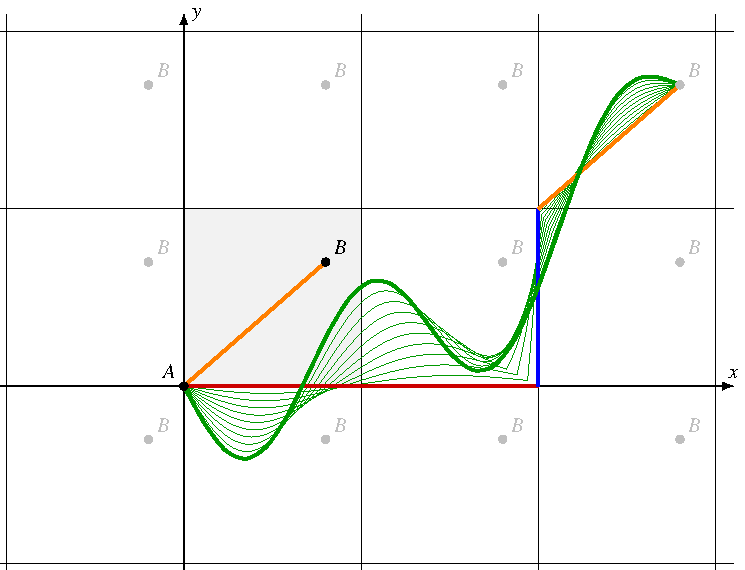
\includegraphics{chapters/120-topologie/images/toruspfade.pdf}
\caption{Ein zweidimensionaler Torus $T$ wird beschrieben als 
Punkte der zweidimensionalen Ebene.
Zwei Punkte werden gleich betrachtet,
wenn sich ihre Koordinaten um eine Ganzzahl unterscheiden.
\index{Torus}%
Alle eingezeichneten Punkte $B$ in der Ebenen stellen also den gleichen
Punkt auf dem Torus dar, sie heissen auch Repräsentanten von $B$.
Ein Weg von $A$ zu $B$ im Torus ist ein Weg von $A$ zu einem beliebigen
Repräsentanten von $B$ in der Ebene.
Jeder solche Pfad ({\color{darkgreen}grün}) kann zerlegt werden in
einen Pfad, der zunächst aus Segmenten ganzzahliger Länge parallel
zur $x$-Achse ({\color{darkred}rot}) bzw.~zur $y$-Achse
({\color{blue}blau}) besteht, gefolgt von einem Segment zum Punkt
$B$ in einem einzelnen Quadrat der Ebene ({\color{orange}orange}).
\label{buch:topologie:kohomologie:fig:toruspfade}}
\end{figure}
